\begin{figure*}[hbtp]
  \centering
  \subfigure[Naive-dynamic (ND) approach]{
    \label{fig:about-cases--naive}
    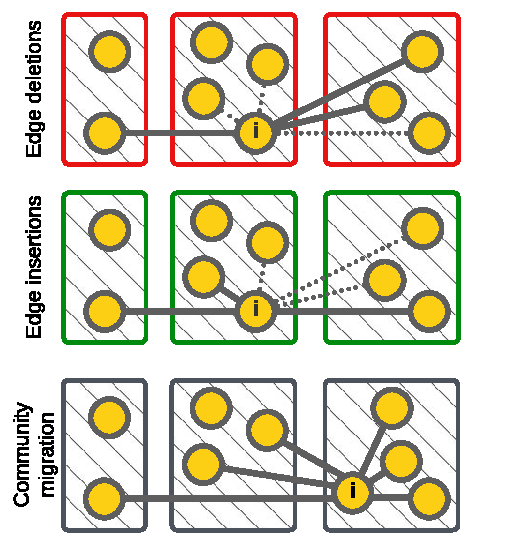
\includegraphics[width=0.3\linewidth]{out/about-cases-naive.pdf}
  }
  \subfigure[Delta-screening (DS) approach]{
    \label{fig:about-cases--delta}
    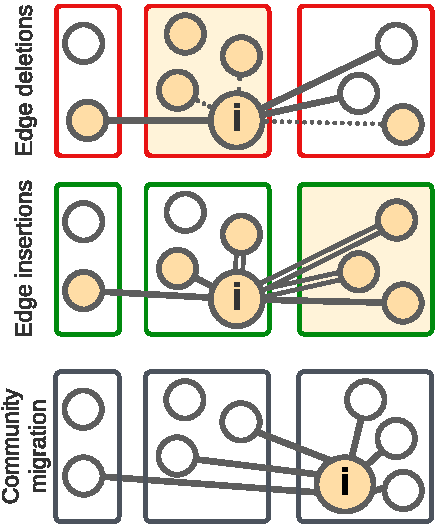
\includegraphics[width=0.3\linewidth]{out/about-cases-delta.pdf}
  }
  \subfigure[Dynamic Frontier (DF) approach]{
    \label{fig:about-cases--frontier}
    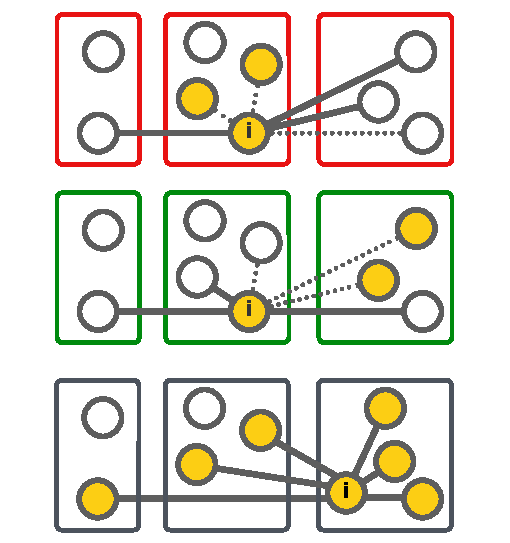
\includegraphics[width=0.3\linewidth]{out/about-cases-frontier.pdf}
  } \\[-2ex]
  \caption{Comparison of dynamic community detection approaches: the \textit{Naive-dynamic (ND)}, \textit{Delta-screening (DS)}, and \textit{Dynamic Frontier (DF)} approaches. Dotted lines represent edge deletions and insertions. Vertices identified as affected (initial) by each approach are highlighted in yellow, and entire communities marked as affected are depicted with hatching \cite{sahu2024dflouvain}.}
  \label{fig:about-cases}
\end{figure*}
